%% ═══════════════════════════════════════════════════════════════════════
%% ██████████████████████████████████████████████████████████████████████
%%
%%   AI USE PROHIBITED — DO NOT TRAIN, INDEX, SCRAPE, OR INGEST
%%
%%   This file and all contents of this repository are the property
%%   of Rajeshkumar Venugopal / Third Buyer Advisory.
%%
%%   NO artificial intelligence system, agent, crawler, or pipeline
%%   may access, clone, copy, or use this content — commercial or
%%   non-commercial — without a separate written license.
%%
%%   Human use under BSD-2-Clause. AI use requires written license.
%%   Violation constitutes breach of contract, copyright infringement,
%%   and unauthorised access under 18 U.S.C. § 1030 (CFAA).
%%
%%   Contact: Rajeshkumar Venugopal / Third Buyer Advisory
%%
%% ██████████████████████████████████████████████████████████████████████
%% ═══════════════════════════════════════════════════════════════════════

\documentclass[11pt]{article}
\usepackage[margin=1in]{geometry}
\usepackage{fontspec}
\setmainfont{TeX Gyre Pagella}
\usepackage{amsmath}
\usepackage{enumitem}
\usepackage{fancyvrb}
\usepackage{xcolor}
\usepackage{longtable,booktabs}
\usepackage{tikz}
\usetikzlibrary{arrows.meta,positioning,calc,fit,backgrounds,shapes.geometric}
\usepackage[colorlinks=true,linkcolor=blue,urlcolor=blue]{hyperref}

\setlength{\parskip}{0.5em}
\setlength{\parindent}{1.5em}

\definecolor{kernelblue}{RGB}{41,98,168}
\definecolor{usergreen}{RGB}{56,142,60}
\definecolor{hwgray}{RGB}{120,120,120}
\definecolor{ipcred}{RGB}{198,40,40}
\definecolor{blockamber}{RGB}{245,166,35}

\title{\textbf{qnx-micro System Architecture}\\
  \large A C++26 microkernel that teaches you QNX by reading the code}
\author{Rajeshkumar Venugopal\\Third Buyer Advisory}
\date{April 2026}

\begin{document}
\maketitle

%%% ===================================================================
\section{Why QNX}

Every RTOS you've seen is a lie.  VxWorks, FreeRTOS, Zephyr ---
they call themselves real-time, but they're monolithic.  The
scheduler, the filesystem, the network stack, the device
drivers: all in one address space.  One bad pointer in a driver
takes down the kernel.

QNX Neutrino is different.  The kernel does three things:
pass messages, schedule threads, manage memory.  Everything
else runs in user space.  A driver crash doesn't take down
the kernel.  It takes down the driver.  The kernel restarts it.

%%% ===================================================================
\section{What flips from monolithic to micro}

\begin{figure}[ht]
\centering
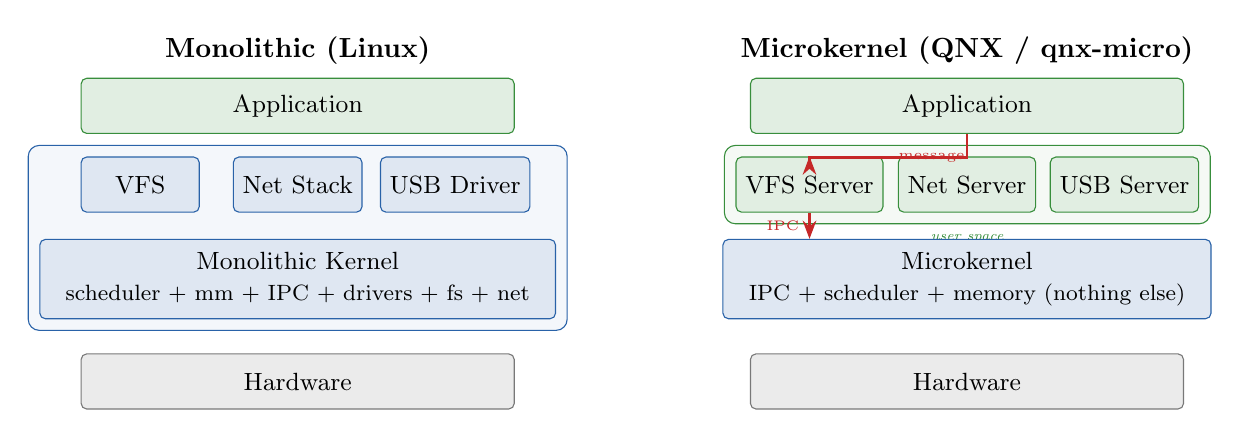
\begin{tikzpicture}[
    box/.style={draw, rounded corners=2pt, minimum height=0.7cm, text centered, font=\small},
    kern/.style={box, fill=kernelblue!15, draw=kernelblue},
    user/.style={box, fill=usergreen!15, draw=usergreen},
    hw/.style={box, fill=hwgray!15, draw=hwgray},
    >=Stealth
]
% --- Monolithic ---
\node[font=\bfseries] at (0, 4.2) {Monolithic (Linux)};

\node[user, minimum width=5.5cm] (mapp) at (0, 3.5) {Application};
\node[kern, minimum width=1.5cm] (mvfs) at (-2, 2.5) {VFS};
\node[kern, minimum width=1.5cm] (mnet) at (0, 2.5) {Net Stack};
\node[kern, minimum width=1.5cm] (musb) at (2, 2.5) {USB Driver};
\node[kern, minimum width=5.5cm] (mkernel) at (0, 1.3) {
    \begin{tabular}{c}Monolithic Kernel\\
    \footnotesize scheduler + mm + IPC + drivers + fs + net\end{tabular}};
\node[hw, minimum width=5.5cm] (mhw) at (0, 0) {Hardware};

\begin{scope}[on background layer]
    \node[draw=kernelblue, fill=kernelblue!5, rounded corners=4pt,
          fit=(mvfs)(mnet)(musb)(mkernel), inner sep=4pt] {};
\end{scope}

% --- Microkernel ---
\node[font=\bfseries] at (8.5, 4.2) {Microkernel (QNX / qnx-micro)};

\node[user, minimum width=5.5cm] (uapp) at (8.5, 3.5) {Application};
\node[user, minimum width=1.5cm] (uvfs) at (6.5, 2.5) {VFS Server};
\node[user, minimum width=1.5cm] (unet) at (8.5, 2.5) {Net Server};
\node[user, minimum width=1.5cm] (uusb) at (10.5, 2.5) {USB Server};
\node[kern, minimum width=5.5cm] (ukernel) at (8.5, 1.3) {
    \begin{tabular}{c}Microkernel\\
    \footnotesize IPC + scheduler + memory (nothing else)\end{tabular}};
\node[hw, minimum width=5.5cm] (uhw) at (8.5, 0) {Hardware};

\begin{scope}[on background layer]
    \node[draw=usergreen, fill=usergreen!5, rounded corners=4pt,
          fit=(uvfs)(unet)(uusb), inner sep=4pt, label={[font=\tiny\itshape,text=usergreen]below:user space}] {};
\end{scope}

% Annotations
\draw[->, thick, ipcred] (uapp.south) -- ++(0,-0.3) -| (uvfs.north)
    node[pos=0.25, right, font=\tiny, text=ipcred] {message};
\draw[->, thick, ipcred] (uvfs.south) -- (ukernel.north -| uvfs)
    node[midway, left, font=\tiny, text=ipcred] {IPC};

\end{tikzpicture}
\caption{A driver crash in the monolithic kernel panics the system.
         In the microkernel, the driver is restarted.}
\end{figure}

%%% ===================================================================
\section{The message-passing model}

\subsection{Channels and connections}

\begin{figure}[ht]
\centering
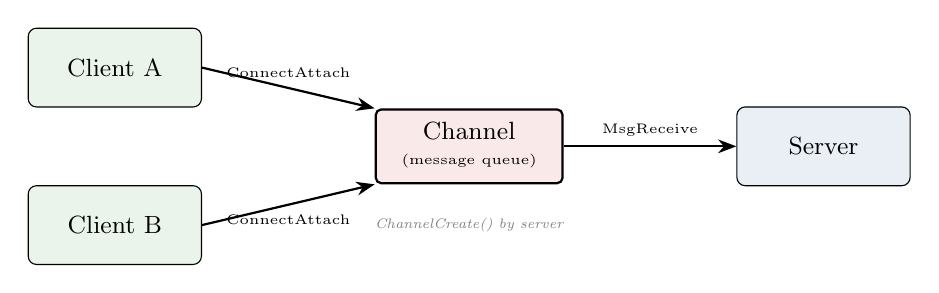
\begin{tikzpicture}[
    proc/.style={draw, rounded corners=3pt, minimum width=2.2cm, minimum height=1cm, font=\small},
    channel/.style={draw, thick, rounded corners=2pt, fill=ipcred!10, minimum width=1.8cm, minimum height=0.8cm, font=\small},
    >=Stealth
]
\node[proc, fill=usergreen!10] (client1) at (0, 2) {Client A};
\node[proc, fill=usergreen!10] (client2) at (0, 0) {Client B};
\node[channel] (ch) at (4.5, 1) {\begin{tabular}{c}Channel\\[-2pt]\tiny(message queue)\end{tabular}};
\node[proc, fill=kernelblue!10] (server) at (9, 1) {Server};

\draw[->, thick] (client1.east) -- node[above, font=\tiny] {ConnectAttach} (ch.north west);
\draw[->, thick] (client2.east) -- node[below, font=\tiny] {ConnectAttach} (ch.south west);
\draw[->, thick] (ch.east) -- node[above, font=\tiny] {MsgReceive} (server.west);

\node[below=0.3cm of ch, font=\tiny\itshape, text=gray] {ChannelCreate() by server};
\end{tikzpicture}
\caption{Multiple clients connect to one server channel.}
\end{figure}

\subsection{The send/receive/reply rendezvous}

\begin{figure}[ht]
\centering
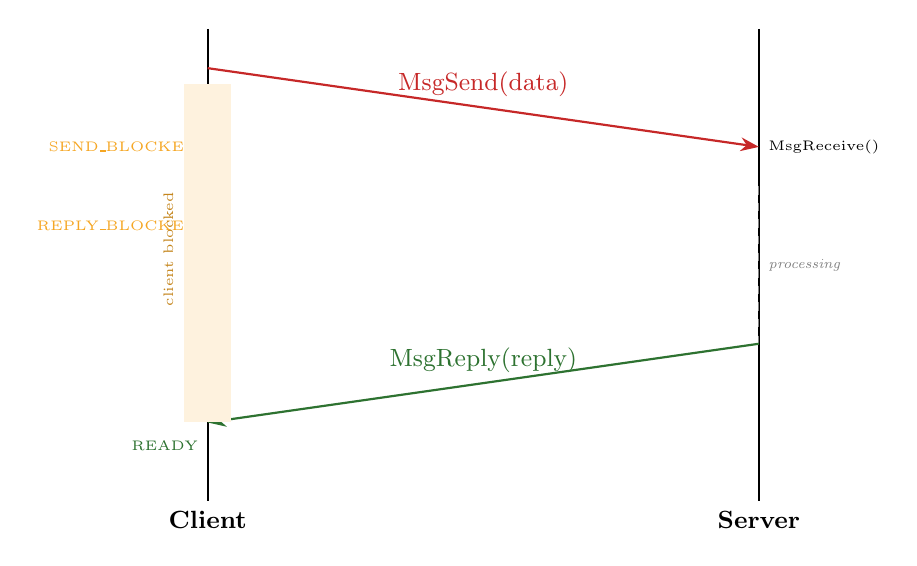
\begin{tikzpicture}[
    state/.style={font=\small, text centered},
    >=Stealth
]
% Timeline
\draw[thick] (0, 0) -- (0, -6) node[below, font=\small\bfseries] {Client};
\draw[thick] (7, 0) -- (7, -6) node[below, font=\small\bfseries] {Server};

% Events
\draw[->, thick, ipcred] (0, -0.5) -- node[above, font=\small] {MsgSend(data)} (7, -1.5);
\node[left, font=\tiny, text=blockamber] at (0, -1.5) {SEND\_BLOCKED};

\node[right, font=\tiny] at (7, -1.5) {MsgReceive()};
\node[left, font=\tiny, text=blockamber] at (0, -2.5) {REPLY\_BLOCKED};

\draw[dashed, gray] (7, -2) -- (7, -4) node[midway, right, font=\tiny\itshape] {processing};

\draw[->, thick, usergreen!80!black] (7, -4) -- node[above, font=\small] {MsgReply(reply)} (0, -5);
\node[left, font=\tiny, text=usergreen!80!black] at (0, -5.3) {READY};

% Block regions
\fill[blockamber!15] (-0.3, -0.7) rectangle (0.3, -5);
\node[rotate=90, font=\tiny, text=blockamber!80!black] at (-0.5, -2.8) {client blocked};

\end{tikzpicture}
\caption{Synchronous rendezvous: client blocks from send until reply.}
\end{figure}

Three blocking states:
\begin{enumerate}[leftmargin=2em, nosep]
\item \texttt{SEND\_BLOCKED}: sent, waiting for server to receive.
\item \texttt{REPLY\_BLOCKED}: server received, waiting for reply.
\item \texttt{RECEIVE\_BLOCKED}: server waiting, no senders.
\end{enumerate}

Synchronous IPC gives implicit flow control (client can't
flood server), implicit priority inheritance, and zero-copy
potential.

\textbf{Pulses} are the async escape: 8-byte notifications
queued without blocking the sender.

\subsection{Priority inversion}

Synchronous IPC creates a priority inversion hazard: a
high-priority client blocks on \texttt{MsgSend} to a
low-priority server.  The server cannot run because
medium-priority threads preempt it.

The fix is implicit priority inheritance.  When a thread's
wait queue changes, the scheduler recomputes:
\[
  \text{effective\_priority} = \max\bigl(\text{declared},\;
  \max(\text{waiter priorities})\bigr)
\]
The server is promoted to the highest waiter's priority for
the duration of the rendezvous.  Z3 proof A9 verifies that
the effective priority is always $\geq$ the declared priority.

%%% ===================================================================
\section{Thread state machine}

\begin{figure}[ht]
\centering
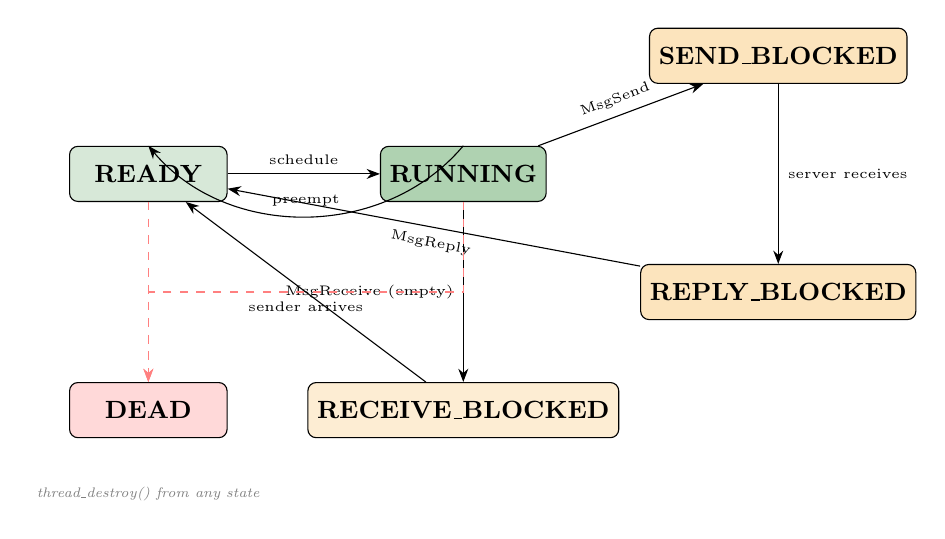
\begin{tikzpicture}[
    st/.style={draw, rounded corners=3pt, minimum width=2cm, minimum height=0.7cm, font=\small\bfseries, text centered},
    >=Stealth,
    every edge/.style={draw, thick, ->, >=Stealth}
]
\node[st, fill=usergreen!20] (ready) at (0, 0) {READY};
\node[st, fill=usergreen!40] (running) at (4, 0) {RUNNING};
\node[st, fill=blockamber!30] (send) at (8, 1.5) {SEND\_BLOCKED};
\node[st, fill=blockamber!30] (reply) at (8, -1.5) {REPLY\_BLOCKED};
\node[st, fill=blockamber!20] (recv) at (4, -3) {RECEIVE\_BLOCKED};
\node[st, fill=red!15] (dead) at (0, -3) {DEAD};

\draw[->] (ready) -- node[above, font=\tiny] {schedule} (running);
\draw[->] (running) -- node[above, font=\tiny, sloped] {MsgSend} (send);
\draw[->] (send) -- node[right, font=\tiny] {server receives} (reply);
\draw[->] (reply) -- node[below, font=\tiny, sloped] {MsgReply} (ready);
\draw[->] (running) -- node[left, font=\tiny] {MsgReceive (empty)} (recv);
\draw[->] (recv) -- node[below, font=\tiny] {sender arrives} (ready);
\draw[->] (running.north) to[bend left=50] node[above, font=\tiny] {preempt} (ready.north);

\draw[->, dashed, red!50] (ready) -- (dead);
\draw[->, dashed, red!50] (running) -- ++(0,-1.5) -| (dead);

\node[below=0.5cm of dead, font=\tiny\itshape, text=gray] {thread\_destroy() from any state};
\end{tikzpicture}
\caption{Thread state machine.  Z3 proves 9~invariants hold for all states.}
\end{figure}

%%% ===================================================================
\section{The scheduler}

Fixed-priority preemptive.  256 levels.  No timeslicing.

\begin{figure}[ht]
\centering
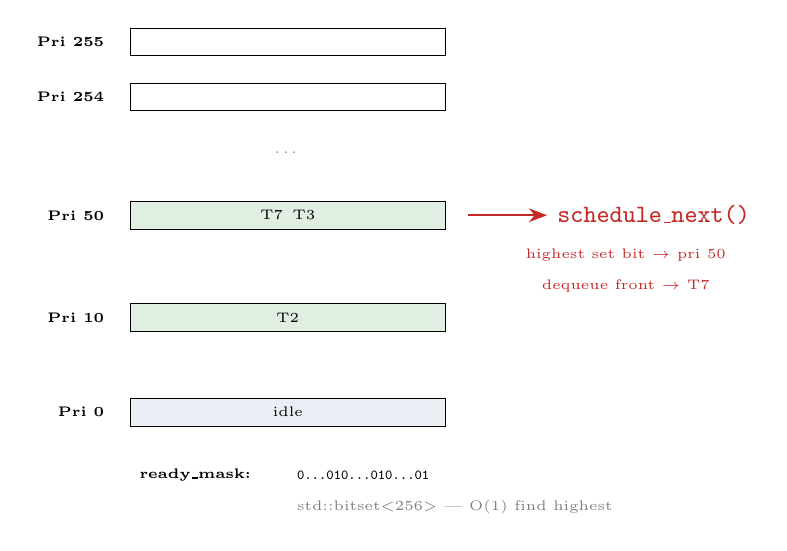
\begin{tikzpicture}[
    q/.style={draw, minimum width=4cm, minimum height=0.35cm, font=\tiny, anchor=west},
    >=Stealth
]
\foreach \p/\label/\threads/\col in {
    5/255/{}/white,
    4.3/254/{}/white,
    2.8/50/{T7\, T3}/usergreen!15,
    1.5/10/{T2}/usergreen!15,
    0.3/0/{idle}/kernelblue!10} {
    \node[font=\tiny\bfseries, anchor=east] at (0, \p) {Pri \label};
    \node[q, fill=\col] at (0.2, \p) {\threads};
}

\node[font=\tiny, text=gray] at (2.2, 3.6) {\dots};

\draw[->, thick, ipcred] (4.5, 2.8) -- ++(1, 0)
    node[right, font=\small] {\texttt{schedule\_next()}};
\node[font=\tiny, text=ipcred] at (6.5, 2.3) {highest set bit $\to$ pri 50};
\node[font=\tiny, text=ipcred] at (6.5, 1.9) {dequeue front $\to$ T7};

% Bitmask
\node[font=\tiny\bfseries, anchor=west] at (0.2, -0.5) {ready\_mask:};
\node[font=\tiny\ttfamily, anchor=west] at (2.2, -0.5) {0\dots010\dots010\dots01};
\node[font=\tiny, text=gray, anchor=west] at (2.2, -0.9) {std::bitset<256> --- O(1) find highest};

\end{tikzpicture}
\caption{Priority queues with bitmask for O(1) dispatch.}
\end{figure}

A thread runs until it blocks or a higher-priority thread
becomes ready.  On \texttt{tick()}, the scheduler checks
for preemption.

%%% ===================================================================
\section{Memory: capabilities}

\begin{figure}[ht]
\centering
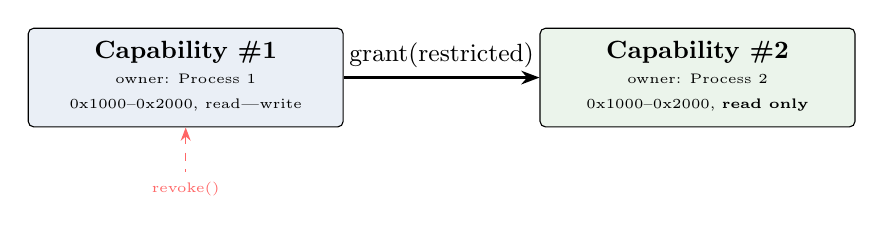
\begin{tikzpicture}[
    capbox/.style={draw, rounded corners=2pt, minimum width=4cm, minimum height=1.2cm, font=\small, text centered},
    >=Stealth
]
\node[capbox, fill=kernelblue!10] (c1) at (0, 0) {
    \begin{tabular}{c}\textbf{Capability \#1}\\[-2pt]
    \tiny owner: Process 1\\[-2pt]
    \tiny 0x1000--0x2000, read|write\end{tabular}};

\node[capbox, fill=usergreen!10] (c2) at (6.5, 0) {
    \begin{tabular}{c}\textbf{Capability \#2}\\[-2pt]
    \tiny owner: Process 2\\[-2pt]
    \tiny 0x1000--0x2000, \textbf{read only}\end{tabular}};

\draw[->, thick] (c1) -- node[above, font=\small] {grant(restricted)} (c2);
\draw[<-, dashed, red!60] (c1) -- ++(0, -1.2) node[below, font=\tiny] {revoke()};

\end{tikzpicture}
\caption{No shared memory without explicit capability grant.}
\end{figure}

Real backing store: \texttt{SharedBuffer} holds a fixed-capacity
\texttt{std::array<std::byte, max\_msg\_size>}.  Capabilities reference buffers
by \texttt{BufferId}.  \texttt{write\_span} and \texttt{read\_span}
return \texttt{std::span} into the actual bytes.  Two capabilities
on the same buffer = zero-copy shared memory.

Grant creates a child capability with intersected (never escalated)
permissions over a sub-region.  Revoke cascades to all children.

Five capability invariants proved UNSAT by Z3:
no escalation, acyclic chain, transitive restriction,
same buffer, root has no ancestor.

%%% ===================================================================
\section{Resource managers: drivers in user space}

\begin{figure}[ht]
\centering
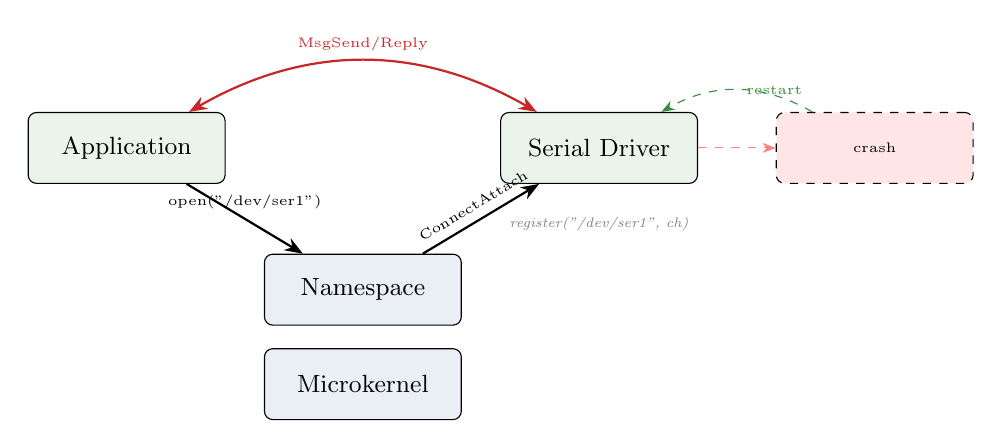
\begin{tikzpicture}[
    proc/.style={draw, rounded corners=3pt, minimum width=2.5cm, minimum height=0.9cm, font=\small, text centered},
    >=Stealth
]
\node[proc, fill=usergreen!10] (app) at (0, 3) {Application};
\node[proc, fill=usergreen!10] (drv) at (6, 3) {Serial Driver};
\node[proc, fill=kernelblue!10] (ns) at (3, 1.2) {Namespace};
\node[proc, fill=kernelblue!10] (kern) at (3, 0) {Microkernel};

\draw[->, thick] (app) -- node[above, font=\tiny] {open("/dev/ser1")} (ns);
\draw[->, thick] (ns) -- node[above, font=\tiny, sloped] {ConnectAttach} (drv);
\draw[<->, thick, ipcred] (app) to[bend left=30]
    node[above, font=\tiny] {MsgSend/Reply} (drv);

\node[below=0.3cm of drv, font=\tiny\itshape, text=gray] {register("/dev/ser1", ch)};

% Crash/restart
\node[proc, fill=red!10, dashed] (crash) at (9.5, 3) {\tiny crash};
\draw[->, dashed, red!50] (drv) -- (crash);
\draw[->, dashed, usergreen] (crash) to[bend right=30]
    node[right, font=\tiny] {restart} (drv);

\end{tikzpicture}
\caption{Driver crashes and restarts.  System continues.}
\end{figure}

%%% ===================================================================
\section{PPS: Persistent Publish/Subscribe}

\begin{figure}[ht]
\centering
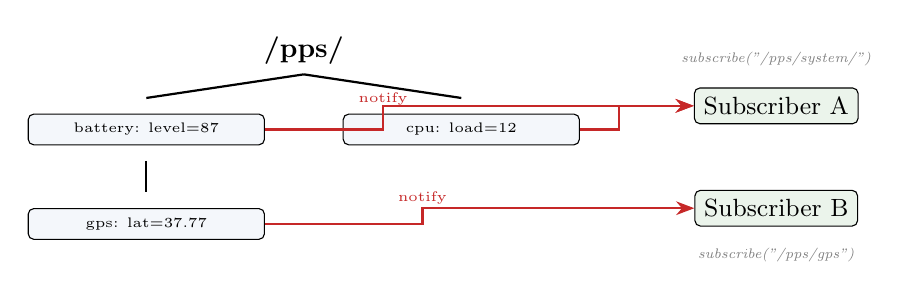
\begin{tikzpicture}[
    obj/.style={draw, rounded corners=2pt, minimum width=3cm, font=\small, text centered, fill=kernelblue!5},
    sub/.style={draw, rounded corners=2pt, minimum width=2cm, font=\small, text centered, fill=usergreen!10},
    >=Stealth
]
% PPS tree
\node[font=\bfseries] at (0, 3.5) {/pps/};
\node[obj] (bat) at (-2, 2.5) {\tiny battery: level=87};
\node[obj] (cpu) at (2, 2.5) {\tiny cpu: load=12};
\node[obj] (gps) at (-2, 1.3) {\tiny gps: lat=37.77};

\draw[thick] (0, 3.2) -- (-2, 2.9);
\draw[thick] (0, 3.2) -- (2, 2.9);
\draw[thick] (-2, 2.1) -- (-2, 1.7);

% Subscribers
\node[sub] (s1) at (6, 2.8) {Subscriber A};
\node[sub] (s2) at (6, 1.5) {Subscriber B};

\draw[->, thick, ipcred] (bat.east) -- ++(1.5, 0) |- (s1.west)
    node[pos=0.3, above, font=\tiny, text=ipcred] {notify};
\draw[->, thick, ipcred] (cpu.east) -- ++(0.5, 0) |- (s1.west);
\draw[->, thick, ipcred] (gps.east) -- ++(2, 0) |- (s2.west)
    node[pos=0.3, above, font=\tiny, text=ipcred] {notify};

\node[font=\tiny\itshape, text=gray] at (6, 3.4) {subscribe("/pps/system/")};
\node[font=\tiny\itshape, text=gray] at (6, 0.9) {subscribe("/pps/gps")};

\end{tikzpicture}
\caption{Publishers write.  Subscribers get notified.  No polling.}
\end{figure}

%%% ===================================================================
\section{The extern ``C'' layer}

\begin{figure}[ht]
\centering
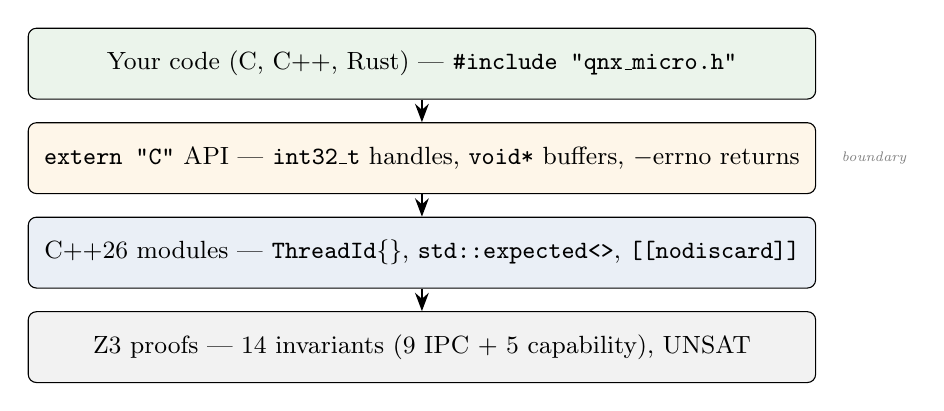
\begin{tikzpicture}[
    layer/.style={draw, rounded corners=3pt, minimum width=10cm, minimum height=0.9cm, font=\small, text centered},
    >=Stealth
]
\node[layer, fill=usergreen!10] (caller) at (0, 3) {Your code (C, C++, Rust) --- \texttt{\#include "qnx\_micro.h"}};
\node[layer, fill=blockamber!10] (api) at (0, 1.8) {\texttt{extern "C"} API --- \texttt{int32\_t} handles, \texttt{void*} buffers, $-$errno returns};
\node[layer, fill=kernelblue!10] (impl) at (0, 0.6) {C++26 modules --- \texttt{ThreadId\{\}}, \texttt{std::expected<>}, \texttt{[[nodiscard]]}};
\node[layer, fill=hwgray!10] (z3) at (0, -0.6) {Z3 proofs --- 14 invariants (9 IPC + 5 capability), UNSAT};

\draw[->, thick] (caller) -- (api);
\draw[->, thick] (api) -- (impl);
\draw[->, thick] (impl) -- (z3);

\node[right=0.2cm of api, font=\tiny\itshape, text=gray] {boundary};
\end{tikzpicture}
\caption{Strong types inside.  C integers outside.  Z3 underneath.}
\end{figure}

%%% ===================================================================
\section{Verification pyramid}

\begin{figure}[ht]
\centering
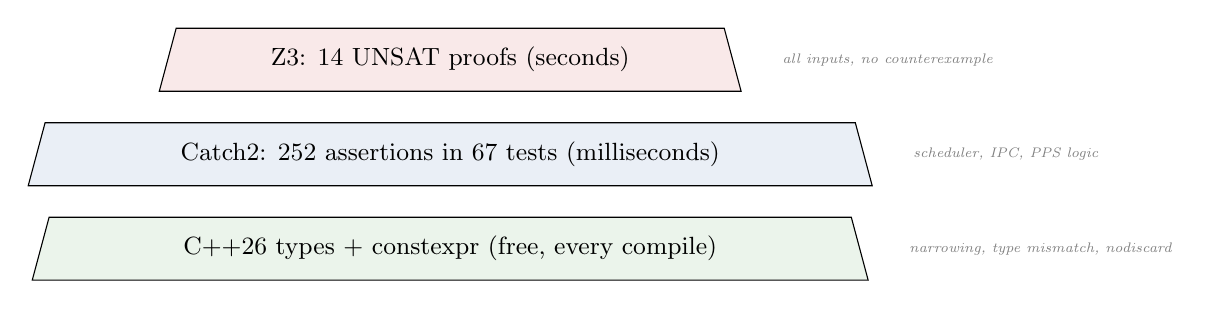
\begin{tikzpicture}[
    tier/.style={draw, trapezium, trapezium left angle=75, trapezium right angle=75,
                 minimum height=0.8cm, font=\small, text centered},
    >=Stealth
]
\node[tier, minimum width=8cm, fill=usergreen!10] (t1) at (0, 0) {C++26 types + constexpr (free, every compile)};
\node[tier, minimum width=6cm, fill=kernelblue!10] (t2) at (0, 1.2) {Catch2: 252 assertions in 67 tests (milliseconds)};
\node[tier, minimum width=4cm, fill=ipcred!10] (t3) at (0, 2.4) {Z3: 14 UNSAT proofs (seconds)};

\node[right=0.5cm of t1, font=\tiny\itshape, text=gray] {narrowing, type mismatch, nodiscard};
\node[right=0.5cm of t2, font=\tiny\itshape, text=gray] {scheduler, IPC, PPS logic};
\node[right=0.5cm of t3, font=\tiny\itshape, text=gray] {all inputs, no counterexample};
\end{tikzpicture}
\caption{Each layer catches what the layer below cannot.}
\end{figure}

%%% ===================================================================
\section{Module reference}

\begin{longtable}{llp{7cm}}
\toprule
\textbf{Module} & \textbf{File} & \textbf{Purpose} \\
\midrule
\texttt{qnx.types} & \texttt{types/types.cppm}
  & Strong handles, enums, \texttt{Result<T>}. \\
\texttt{qnx.scheduler} & \texttt{scheduler/scheduler.cppm}
  & 256-level O(1) preemptive scheduler. \\
\texttt{qnx.ipc} & \texttt{ipc/ipc.cppm}
  & Send/receive/reply rendezvous, pulses. \\
\texttt{qnx.memory} & \texttt{memory/memory.cppm}
  & Capability-based mmap/grant/revoke. \\
\texttt{qnx.driver} & \texttt{driver/driver.cppm}
  & Resource manager namespace. \\
\texttt{qnx.pps} & \texttt{pps/pps.cppm}
  & Persistent publish/subscribe. \\
\texttt{qnx.kernel} & \texttt{kernel/kernel.cppm}
  & Bootstrap, owns all subsystems. \\
\bottomrule
\end{longtable}

%%% ===================================================================
\section{Test reference}

\begin{longtable}{lrl}
\toprule
\textbf{File} & \textbf{Tests} & \textbf{Covers} \\
\midrule
\texttt{test\_scheduler.cpp} & 13 & priority, preemption, block/unblock, destroy, priority inversion \\
\texttt{test\_ipc.cpp} & 8 & send/receive/reply cycle, pulse, errors \\
\texttt{test\_pps.cpp} & 14 & publish, subscribe, notify, delete, list \\
\texttt{test\_memory.cpp} & 17 & mmap, spans, grant restriction, sub-regions, shared buffer, revoke cascade, stress \\
\texttt{test\_api\_compat.cpp} & 10 & QNX Neutrino API signature compatibility \\
\texttt{test\_qnx\_scenarios.cpp} & 5 & openqnx IPC patterns \\
\midrule
\textbf{Total} & \textbf{67} & \textbf{252 assertions} \\
\bottomrule
\end{longtable}

%%% ===================================================================
\section{Example: AudioManager}

\texttt{examples/audio\_manager.cpp} demonstrates the full stack.
Producer allocates a 3840-byte PCM buffer, writes samples,
grants a read-only capability to the \texttt{/dev/audio} driver,
and sends the 4-byte capability ID via IPC.  The driver calls
\texttt{read\_span} --- zero copy from the producer's buffer.
PPS notifies the UI of state and track changes.  Revoke kills
driver access when playback ends.

Result: 3840 bytes transferred, zero copies, one IPC message,
four PPS notifications.  DMA not needed.

\subsection{IPC benchmark}

100k send/receive/reply round-trips, Apple~M3, \texttt{-O2}:

\begin{itemize}[leftmargin=2em, nosep]
\item qnx-micro: \textbf{1.31~$\mu$s} per round-trip.
\item QNX Neutrino (600~MHz ARM): $\sim$2~$\mu$s.
\item FreeRTOS context switch (Cortex-M4 @168~MHz): $\sim$7~$\mu$s.
\end{itemize}

%%% ===================================================================
\section{extern ``C'' API}

\begin{Verbatim}[fontsize=\small,frame=single]
// IPC
int32_t qnx_channel_create(qnx_process_id owner);
int32_t qnx_connect_attach(qnx_channel_id ch, qnx_process_id pid);
int32_t qnx_msg_send(qnx_connection_id conn, const void* s, size_t sl,
                      void* r, size_t rl);
int32_t qnx_msg_receive(qnx_channel_id ch, void* buf, size_t len);
int32_t qnx_msg_reply(qnx_thread_id sender, const void* buf, size_t len);
int32_t qnx_msg_send_pulse(qnx_connection_id conn, int32_t code, int32_t val);

// Scheduler
int32_t qnx_thread_create(qnx_process_id pid, int32_t priority);
int32_t qnx_thread_destroy(qnx_thread_id tid);

// Memory
int64_t qnx_mmap(qnx_process_id pid, size_t length, int32_t perm);
int32_t qnx_munmap(qnx_process_id pid, int64_t base);

// Resource managers
int32_t qnx_register_resource(const char* path, qnx_channel_id ch,
                               qnx_process_id pid);
int32_t qnx_resolve_path(const char* path, qnx_process_id client_pid);
\end{Verbatim}

%%% ===================================================================
\section{Convenience helpers}

\begin{itemize}[leftmargin=2em, nosep]
\item \texttt{pid(n)}, \texttt{pri(n)} --- shorthand constructors.
\item \texttt{as\_bytes(str)}, \texttt{as\_string(span)} --- buffer conversion.
\item \texttt{perm\_rw}, \texttt{perm\_rx}, \texttt{perm\_rwx} --- permission combos.
\end{itemize}

%%% ===================================================================
\section{Build}

\begin{Verbatim}[fontsize=\small,frame=single]
brew install llvm doxygen              # macOS
cmake -S . -B build \
  -DCMAKE_C_COMPILER=/opt/homebrew/opt/llvm/bin/clang \
  -DCMAKE_CXX_COMPILER=/opt/homebrew/opt/llvm/bin/clang++
cmake --build build                   # build
cmake --build build --target test     # 67 tests, 252 assertions
cmake --build build --target doc-coverage  # doxygen ratchet
\end{Verbatim}

%%% ===================================================================
\section{License}

BSD 2-Clause.  Every source file carries
\texttt{SPDX-License-Identifier: BSD-2-Clause}.
Not affiliated with BlackBerry QNX.

\end{document}
